%=============================================================================%
% Author: 	John Joseph Valletta
% Date: 	23/04/2017
% Title: 	Python workshop: NumPy/SciPy
%=============================================================================%

%=============================================================================%
% Preamble
%=============================================================================%
% Libraries
\documentclass[pdf]{beamer}
\usepackage[export]{adjustbox}
\usepackage{framed}
\usepackage{color}
\definecolor{dkgreen}{rgb}{0,0.6,0}
\definecolor{gray}{rgb}{0.5,0.5,0.5}
\definecolor{mauve}{rgb}{0.58,0,0.82}
\definecolor{deepblue}{rgb}{0,0,0.5}
\definecolor{deepred}{rgb}{0.6,0,0}
\definecolor{deepgreen}{rgb}{0,0.5,0}
\definecolor{lightgray}{rgb}{0.92,0.92,0.92}
\usepackage{listings} % to insert code
\usepackage{textpos} % textblock
\usepackage{dirtree} % to make directory trees
\usepackage{hyperref}
\usepackage{amsmath} 
\hypersetup{colorlinks=true, urlcolor=blue, linkcolor=black} 
\renewcommand{\d}[1]{\ensuremath{\operatorname{d}\!{#1}}} % derivative d

% Listing set up
% Python
\lstdefinestyle{python}{
language=python,
formfeed=\newpage,
basicstyle=\scriptsize\ttfamily,
commentstyle=\color{deepgreen},%\color{gray},
%numbers=left,
%numberstyle=\tiny\color{gray},
stepnumber=1,
numbersep=5pt,
backgroundcolor=\color{lightgray},%\color{white},
showspaces=false,
showstringspaces=false,
showtabs=false,
frame=lines,
tabsize=4,
captionpos=b,
breaklines=true,
breakatwhitespace=false,
title=\lstname,
escapeinside={},
keywordstyle=\color{deepblue},
emphstyle=\color{deepred},
stringstyle=\color{mauve},
morekeywords={as, lambda, None}
}

% Presentation configuration
\mode<presentation>{\usetheme{Madrid}}
\definecolor{tealblue}{rgb}{0, 0.5, 0.5}
\usecolortheme[named=tealblue]{structure}
\useinnertheme{circles} % circles, rectanges, rounded, inmargin
\usefonttheme[onlymath]{serif} % makes math fonts like the usual LaTeX ones
\setbeamercovered{transparent=4} % transparent
\setbeamertemplate{caption}{\raggedright\insertcaption\par} % Remove the word "Figure" from caption %\setbeamertemplate{caption}[default]
\setbeamertemplate{navigation symbols}{} % don't put navigation tools at the bottom (alternatively \beamertemplatenavigationsymbolsempty)
\graphicspath{ {../images/} }

% Titlepage
\title[Python for scientific research]{Python for scientific research}
\subtitle{Number crunching using \texttt{NumPy/SciPy}}
\author{John Joseph Valletta}
\date[June 2017]{June 2017}
\institute[]{University of Exeter, Penryn Campus, UK}
\titlegraphic{
\hfill

\includegraphics[width=\textwidth, keepaspectratio]{logo.jpg}}

%=============================================================================%
%=============================================================================%
% Start of Document
%=============================================================================%
%=============================================================================%
\begin{document}

%=============================================================================%
%=============================================================================%
\begin{frame}
\titlepage
\end{frame}

%=============================================================================%
%=============================================================================%
\begin{frame}{What we've done so far}

	\begin{enumerate}\addtolength{\itemsep}{1\baselineskip}
		\item Declare variables using built-in data types and execute operations
		on them
		\item Use flow control commands to dictate the order in which commands are run
		and when
		\item Encapsulate programs into reusable functions, modules and packages
		\item \textbf{Next}: Number crunching using \texttt{NumPy/SciPy}
	\end{enumerate}

\end{frame}

%=============================================================================%
%=============================================================================%
\begin{frame}{Motivation}

\begin{itemize}\addtolength{\itemsep}{\baselineskip}
	\item<1-> We are typically faced by numerical tasks, 
	such as, computing Pearson's correlation coefficient
	or generating random numbers

	\item<2-> The \texttt{NumPy} (numeric python) package provides
	a comprehensive set of mathematical data structures (e.g vector, matrix)
	and functions (e.g trigonometry, random number generator) 

	\item<3-> The \texttt{SciPy} (scientific python) library builds on top
	of \texttt{NumPy} to provide a collection of numerical algorithms for: 
	\begin{itemize}
		\item<4-> Statistics (e.g correlation coefficient)
		\item<5-> Signal processing (e.g Fourier transform, filtering)
		\item<6-> Solving differential equations
		\item<7-> Optimisation
		\item<8-> $\ldots$
	\end{itemize}
\end{itemize}
\end{frame}

%=============================================================================%
%=============================================================================%
\begin{frame}[fragile]
\frametitle{A taste of NumPy}

\begin{lstlisting}[style=python]
import numpy as np

# 1D array/vector
x = np.array([1, 2, 3, 4])
x.min() # return min of array 
x.max() # return max of array
x.sum() # sum all elements in array

# 2D array
x = np.array([[1, 2, 3], [4, 5, 6], [7, 8, 9]])
x*x # element-by-element multiplication
x.shape # return dimensions of matrix
np.dot(x, x) # matrix multiplication
np.mat(x)*np.mat(x) # matrix multiplication (cast as matrix)
\end{lstlisting}

\end{frame}

%=============================================================================%
%=============================================================================%
\begin{frame}[fragile]
\frametitle{A taste of NumPy}

\begin{lstlisting}[style=python]
# Generate random numbers
np.random.rand() # from a uniform distribution
np.random.randn() # from a normal distribution
np.random.randn(5, 5) # 5 x 5 matrix of random numbers

# Create number sequences
np.arange(0, 1, 0.1) # 0 to 1 in steps of 0.1
np.linspace(0, 1, 100) # 100 values between 0 and 1
np.logspace(0, 1, 10) # 10 values between 10^0 and 10^1
\end{lstlisting}

\end{frame}

%=============================================================================%
%=============================================================================%
\begin{frame}[fragile]
\frametitle{A taste of SciPy}

\begin{lstlisting}[style=python]
import scipy.stats as sp

# Create two random arrays
x1 = np.random.randn(30)
x2 = np.random.randn(30)

# Correlation coefficientss
sp.pearsonr(x1, x2) # pearson correlation
sp.spearmanr(x1, x2) # spearman correlation
sp.kendalltau(x1, x2) # kendall correlation

# Statistical tests
sp.ttest_ind(x1, x2) # independent t-test
sp.mannwhitneyu(x1, x2) #  Mann-Whitney rank test 
sp.wilcoxon(x1, x2) # Wilcoxon signed-rank test

# Least-squares regression
sp.linregress(x1, x2)
\end{lstlisting}

\end{frame}

%=============================================================================%
%=============================================================================%
\begin{frame}[fragile]
\frametitle{Predator prey equations (Lotka Volterra)}

%Prey population = growth rate - rate at which it is preyed
%Predator population = - natural death + food supply

\begin{align*}
 \frac{\d{u}}{\d{t}} &= \alpha u - \beta uv\\[1em]
\frac{\d{v}}{\d{t}} &= -\gamma v + \delta uv 
\end{align*}

% \begin{align*}
% \text{Prey population:}& \frac{\d{u}}{\d{t}} &=& \underbrace{\alpha u}_\text{own growth rate} - \underbrace{\beta uv}_\text{rate at which it's preyed upon}\\
% \text{Prey population:}& \frac{\d{v}}{\d{t}} &=& \underbrace{-\gamma v}_\text{natural death of predators} + \underbrace{\delta uv}_\text{growth of predator population} 
% \end{align*}




Where:

\begin{itemize}
\item $u$: is the number of prey (e.g rabbits)
\item $v$: is the number of predators (e.g foxes)
%$\frac{\d{x}}{\d{t}}$: prey population growth rate\\
%$\frac{\d{y}}{\d{t}}$: predator population growth rate\\
\item $\alpha$: prey growth rate in the absence of predators
\item $\beta$: dying rate of prey due to predation
\item $\gamma$: dying rate of predators in the absence of prey
\item $\delta$: predator growth rate when consuming prey
\end{itemize}

% Prey population = growth rate - rate at which it is preyed
% Predatory population = - natural death + food supply

\end{frame}

%=============================================================================%
%=============================================================================%
\begin{frame}[fragile]
\frametitle{Predator prey equations in Python}

\vspace{-0.4cm}
\scriptsize
\begin{align*}
 \frac{\d{u}}{\d{t}} &= \alpha u - \beta uv\\[0.5em]
\frac{\d{v}}{\d{t}} &= -\gamma v + \delta uv 
\end{align*}
\normalsize


\begin{lstlisting}[style=python]
def predator_prey(x, t):
    """
	Predator prey model (Lotka Volterra)
    """
    # Constants
    alpha = 1
    beta = 0.1
    gamma = 1.5
    delta = 0.075
    
    # x = [u, v] describes prey and predator populations
    u, v = x
    
    # Define differential equation (u = x[0], v = x[1])
    du = alpha*u - beta*u*v
    dv = -gamma*v + delta*u*v
    
    return du, dv
\end{lstlisting}

\end{frame}

%=============================================================================%
%=============================================================================%
\begin{frame}[fragile]
\frametitle{Solve differential equations}

\begin{lstlisting}[style=python] 
from scipy.integrate import odeint

time = np.linspace(0, 35, 1000) # time vector
init = [10, 5] # initial condition: 10 prey, 5 predators
x = odeint(predator_prey, init, time) # solve
\end{lstlisting}

\vspace{-.8cm}

\visible<2->{
\begin{center}
	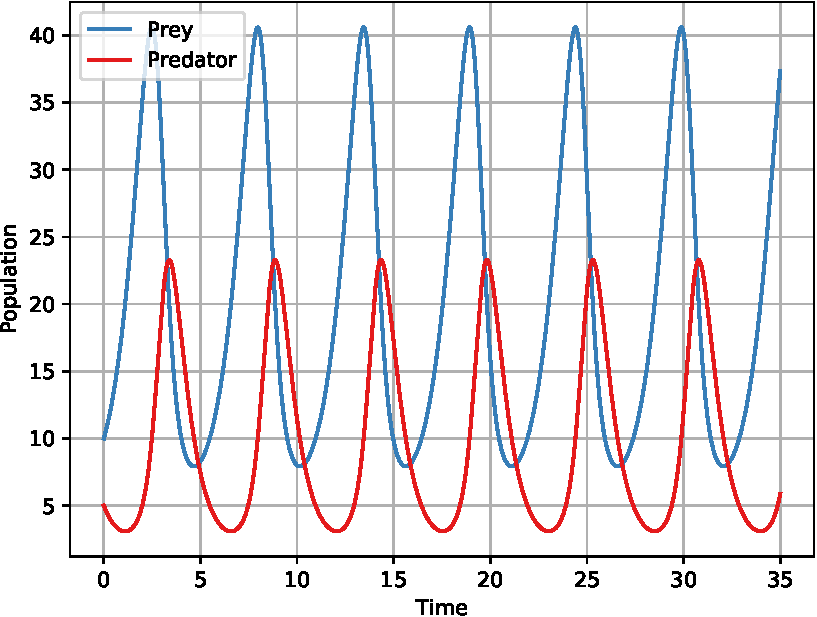
\includegraphics[width=.65\textwidth]{predator_prey.pdf}
\end{center}}

\end{frame}

%=============================================================================%
%=============================================================================%
\begin{frame}[fragile]
\frametitle{Fourier transform}

\begin{lstlisting}[style=python]
from scipy.fftpack import fftfreq, fft

# Create frequency vector
N = len(time)
freq = fftfreq(N, np.mean(np.diff(time)))
freq = freq[range(int(N/2))]

# Compute Fast Fourier Transform
y = fft(x[:, 0])/N # compute and normalise fft
y = y[range(int(N/2))] # keep only positive frequencies
\end{lstlisting}

\end{frame}

%=============================================================================%
%=============================================================================%
\begin{frame}[fragile]
\frametitle{Fourier transform}

\begin{center}
	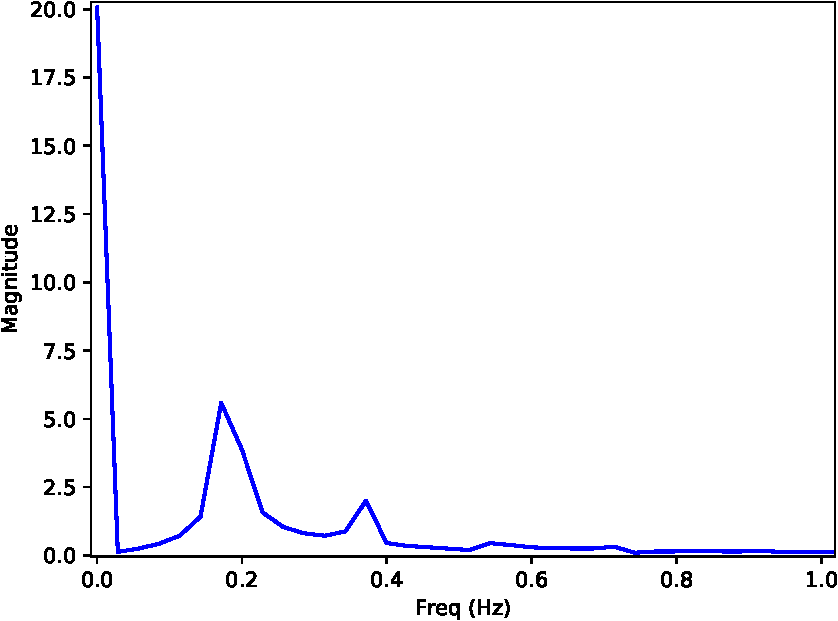
\includegraphics[width=.8\textwidth]{fourier.pdf}
\end{center}

\end{frame}

%=============================================================================%
%=============================================================================%
% End of Document
%=============================================================================%
%=============================================================================%
\end{document}
